\section{Bayesian Seroprevalence Analysis with Seroreversion Correction}
In a serial seroprevalence study conducted in Quebec, Canada by \cite{lewin2021sars} and \cite{lewin2022seroprevalence}, a procedure for seroreversion correction is applied in a non-Bayesian analysis. Here we begin by describing the dataset used in this analysis before illustrating the procedure used to adjust estimated cumulative incidences for seroreversion.
\subsection{Data}
The datasets used in \cite{lewin2021sars} and \cite{lewin2022seroprevalence} together can be viewed as one for a serial COVID-19 seroprevalence study in Quebec, Canada. For both phases of the study, numbers of antibody-positive samples as well as total number of samples are recorded for each of the three regions in Quebec: Montreal-Laval region, region surrounding Montreal-Laval, as well as other regions. Phase I of the study was conducted relatively early in the pandemic, and it collected samples obtained between May 25 and July 9, 2020. Phase II of the study contains samples collected from  January 25 to Mar 11, 2021.\\
\newline $ $
While we can use the data from phase I of the study to estimate regional cumulative incidences in Quebec between the beginning of the pandemic until around May 23, 2020 (accounting for the average 25 days between infection and when antibodies become detectable), simply repeating the same analysis using data from phase II of the study likely would not result in valid estimates of cumulative incidences between the beginning of the pandemic and the beginning of 2021. This is because there had already been almost a year since the beginning of the pandemic by the time when phase II samples were collected. Some of the individuals may have had a previous infection but had seroreverted by the time of sample collection. Consequently, the raw estimate may be lower than the true cumulative incidence of a given region. As a result, to account for seroreversion when analyzing data from phase II of the seroprevalence study, \cite{lewin2022seroprevalence} also conducted a seroreversion substudy. In particular, a number of the individuals who tested postive for SARS-Cov-2 antibodies during phase I of the study were tested again in 2021. The number of these individuals as well as the number of negative tests (indicating seroreversion) were recorded. The data from both phases of the study are summarized in \cref{tab:dat}.\\
\newline $ $
It is important to point out that the phase II data presented here only concern the unvaccinated population. While data for both those who were and were not vaccinated are presented in \cite{lewin2022seroprevalence}, we have chosen to focus on the unvaccinated population since none of the vaccinated individuals had seroreverted at the time and so it is not necessary for adjust for seroreversion. Finally, we note that for the remainder of the report, any notation that is redefined from the previous sections are within the context of the seroprevalence study in Quebec.

\begin{table}[]
\centering
\begin{tabular}{c|cc|cc|cc}
                           & \multicolumn{2}{c}{\textbf{Phase I}} & \multicolumn{2}{c}{\textbf{Phase II (unvaccinated)}} & \multicolumn{2}{c}{\textbf{Seroreversion substudy}}\\
                           & reactive      & tested      & reactive              & tested      & seroreverted              & tested        \\
                           \hline
Montreal-Laval             & 90            & 3061        & 48                    & 1925      & - & -          \\
Surrounding Montreal-Laval & 48            & 1925        & 128                   & 1422   & - & -             \\
Other                      & 35            & 2705        & 372                   & 4304          & - & -      \\
\hline
Total                      & 173           & 7691        & 715                   & 7304          &    32 & 109  
\end{tabular}
\caption{Seroprevalence data from \cite{lewin2021sars} and \cite{lewin2022seroprevalence}. Reactive indicates the number of positive tests against SARS-Cov-2 IgG.}
\label{tab:dat}
\end{table}
\subsection{Adjusting for seroreversion}\label{sec:adjust_reversion}
As mentioned above, not correcting for seroreversion when conducting seroprevalence analysis on data from phase II of the above-mentioned study may result in unreliable estimates of regional cumulative incidences. This is because such analyses fail to account for those who have had a previous infection but had already seroreverted by the time of sample collection. Luckily, with the data from phase I of the study, for each region in Quebec, we can produce a valid estimate of the cumulative incidence between the beginning of the pandemic and May 2020. Additionally, from the seroreversion substudy, we can estimate the proportion of the antibody-positive population from phase I of the study that had seroreverted by phase II of the study. As a result, \cite{lewin2022seroprevalence} adjusts the raw estimate of cumulative incidence from phase II by adding the product of the estimated cumulative incidence from phase I and the estimated proportion that have seroreverted. Mathematically, let $\hat{s}_{prev}$ be the estimated cumulative incidence of a region in Quebec from phase I, $\hat{p}$ be the estimated observed prevalence (proportion of positive samples) from phase II, and $\hat{sr}$ be the observed proportion of seroreversion, we can estimate the cumulative incidence between the beginning of the pandemic and the beginning of 2021 using
\[
\hat{s} = \hat{p} + \hat{s}_{prev} \times \hat{sr}.
\]
To quantify the uncertainty around $\hat{s}$, we begin by noting that there are three sources of uncertainty: the estimated cumulative incidence from phase I, the observed prevalence from phase II, and the proportion of seroreversion. Note that here the cumulative incidence from phase I is directly estimated using the observed prevalence from phase I. We can construct individual 95\% confidence intervals for the cumulative incidence from phase I $s_{prev}$ and observed prevalence from phase II $p$, as well as the proportion of seroreversion $sr$. We write these intervals as
\[
[s_{prev, l},\quad s_{prev, u}], \quad [p_{l},\quad p_{u}], \quad [sr_{l},\quad sr_{u}].
\]
Then to construct an uncertainty interval for $s$, we can follow \cite{meyer2022adjusting} and aggregate the above three 95\% confidence intervals using combinations of the confidence interval endpoints that give the lowest and highest estimated cumulative incidence
\[
[p_l + s_{prev, l} \times sr_{l}, \quad p_u + s_{prev, u} \times sr_{u}].
\]
Again, the above interval is not a valid $95$\% confidence interval, but it nonetheless quantifies the scale of uncertainty.\\
\newline$ $
We can easily extend the model above and incorporate adjustments for test-kit performance. This is achieved by writing, with $p_{prev}$ denoting the observed prevalence in phase I,
\[
p_{prev} = s_{prev} \times se + (1-s_{prev}) \times (1 - sp) &\implies s_{prev} = \frac{p_{prev} + sp - 1}{se + sp - 1},\\
p = (s - sr \times s_{prev}) \times se + (1 - (s - sr \times s_{prev})) \times (1 - sp) &\implies s = \frac{p+1-sp}{se+sp-1} + sr \times s_{prev}.
\]
In this above formulation of observed prevalence from phase II ($p$), we first substract from the true cumulative incidence the proportion that have seroreverted from the true seroprevalence, and then adjust for test-kit performance. This is because the test-kit only has a chance at detecting antibodies if the subject has not yet seroreverted. Using the same approach to aggregate over all sources of uncertainty, we arrive at the estimated cumulative incidence for a given region between the beginning of the pandemic and the beginning of 2021
\[
\hat{s} = \frac{\hat{p}+1-\hat{sp}}{\hat{se}+\hat{sp}-1} + \hat{sr} \times \hat{s}_{prev}
\]
with a corresponding uncertainty interval adjusting for both seroreversion and test-kit performance
\[
\left[\frac{p_l+1-sp_l}{se_u+sp_l-1} + sr_l \times s_{prev,l}, \quad \frac{p_u+1-sp_u}{se_l+sp_u-1} + sr_u \times s_{prev, u} \right],\\
\]
Note that
\[
s_{prev,l} = (p_{prev,l} + sp_l - 1) / (se_u - 1 + sp_l), \quad s_{prev,u} = (p_{prev,u} + sp_u - 1) / (se_l - 1 + sp_u)
\]
correspond to the 95\% confidence interval endpoints for $s_{prev}$. Finally, we note that if we had data on the unvaccinated population from each of the three regions in Quebec, we could obtain a province-wide estimate of the cumulative incidence by averaging the regional cumulative incidences weighted by the proportion of population in each region. However, this information is not included in \cite{lewin2022seroprevalence}, and so our analysis here remains regional. We also do not adjust for age and sex of individuals due to data unavailability.

\subsection{Model formulation}
While the previous section outlines an approach to conducting seroprevalence analysis that accounts for both seroreversion and test-kit performance, we note that the resulting uncertainty intervals are not valid 95\% confidence intervals, and that it is still possible to get negative estimates in certain cases. As demonstrated in \cite{meyer2022adjusting}, this can be addressed by constructing a Bayesian version of the same analysis. We outline this model below.\\
\newline $ $
Recall that $sr$ denotes the test seroreversion proportion. Following the same notations as established in \cref{sec:approach}, with $i=1,2$ indicating the phase of the study, and $j=1,2,3$ representing Montreal-Laval, surrounding Montreal-Laval, and other regions, the final Bayesian model can be written as
\[
s_{1j} &\sim \distBeta(1,1) \quad \forall j \in \{1,2,3\}\\
s_{2j} &\sim \distBeta(1, 1)_{\{ sr \times s_{1j} , 1 \}} \quad \forall j \in \{1,2,3\}\\
se &\sim \distBeta(205, 29)\\
sp &\sim \distBeta(288, 2)\\
sr &\sim \distBeta(32, 77)\\
p_{1j} &= s_{1j} \times se + (1 - s_{1j}) \times (1 - sp) \quad \forall j \in \{1,2,3\}\\
p_{2j} &= (s_{2j} - sr \times s_{1j}) \times se + (1 - (s_{2j} - sr \times s_{1j})) \times (1 - sp) \quad \forall j \in \{1,2,3\}\\
x_{ij} \given n_{ij}, p_{ij} &\distind \distBinom(n_{ij}, p_{ij}), \quad \forall i \in\{1,2\}, \quad j \in \{1,2,3\}.
\]
The density of the target posterior distribution is then given by
\[
p(S, se, sp, sr \given X, N) = \frac{1}{Z}p(se)p(sp)p(sr)\prod_{i=1}^3\prod_{j=1}^2 p(s_{ij})p(x_{ij}\given sp, se, sr, s_{ij}).
\]
In this above model, $p_{1j}$ is modeled in the same way as \cite{meyer2022adjusting} for all $j$, since there is no need to adjust for seroreversion. $p_{2j}$, on the other hand, accounts for both seroreversion and test-kit performance. Since the population data by the three regions in Quebece are not provided in \cite{lewin2022seroprevalence}, non-informative priors are used here. To ensure we do not run into negative seroprevalence estimates, we truncate $s_{21}, s_{22}, s_{23}$ accordingly. For the priors on test sensitivity and test specificity, we use the untruncated version of the same priors as in \cite{meyer2022adjusting}. This allows for more room for uncertainty given that these tests were conducted at a different location and at different times. Finally, the prior on seroreversion is chosen so that the mean reflects the sample proportion of seroreversion.\\
\newline$ $
Similar to \cite{meyer2022adjusting}, we use MCMC to obtain samples from the target posterior distribution. Specifically, samples from $s_{2j}$ for all $j$ allow us to estimate the regional cumulative incidences in Quebec between the beginning of the pandemic and the beginning of 2021, where the estimates are adjusted for both seroreversion and test-kit performance. \cref{fig:local_trace,fig:global_trace} show that the MCMC algorithm has converged (this is also confirmed by checking the Gelman-Rubin diagnostic). We follow \cite{meyer2022adjusting} and samples from four individual chains ($100,000$ samples each with $100,000$ burn-in samples discarded) to obtain the median as a point estimate as well as the equal-tailed 95\% credible interval for uncertainty quantification.\\
\newline$ $
To compare the Bayesian model output, we also conduct a number of frequentist seroprevalence analyses on the same dataset. In particular, we include the raw estimates of regional cumulative incidence from phase II directly from the sample proportion of positive tests, an analysis that adjusts for seroreversion, as well as an analysis that adjusts for both seroreversion and test-kit performance. The last two analyses correspond to those described in \cref{sec:adjust_reversion}. The code used to generate all results and figures can be found at \url{https://github.com/NaitongChen/QP-4}.

\subsection{Discussion of analysis results}
The estimated regional cumulative incidences as well as their corresponding uncertainty intervals from each of the four analyses are summarized in \cref{tab:results}. We see that from each of the four analyses, the estimated cumulative incidence in the Montreal-Laval region is the highest, and those of the other two regions are similar to each other, with the region surrounding Montreal-Laval having a slightly higher estimated cumulative incidence. We now look at the estimate for the same region across the three non-Bayesian analyses. Going from the raw results to those adjusted for seroreversion, we see that there is an increase in the estimated cumulative incidence. By further adjusting for test-kit performance, we see yet another increase in the estimated cumulative incidence for the same region. This two-step increase is consistently observed for each of the three regions in Quebec. This pattern is sensible as with each additional adjustment, we are inherently adding to the cumulative incidence estimate by including parts of the population that previously would not have been considered. However, as we increase the number of items that we adjust for (seroreversion and test-kit performance), we also incur more sources of uncertainty. Given that we have constructed our uncertainty intervals using the combination of individual 95\% confidence interval endpoints that yield the lowest and highest estimates, the resulting intervals grow wider and wider. Take the Montreal-Laval region as an example, the width of the uncertainty interval increases from $0.34$ in the raw results to $0.113$ in the analysis that accounts for both seroreversion and test-kit performance. The width of the interval more than triples. It is worth mentioning that the uncertainty intervals for $s_{prev}$ for each region (or equivalently $s_{11}, s_{12}, s_{13}$) cross zero. In other words, they contain a negative lowerbound.\\
\newline$ $
We now turn our attention to the output of the Bayesian model. Since the priors for each parameter of interest are properly set up, none of the estimates are negative (\cref{fig:local_trace,fig:global_trace}). Compared to the non-Bayesian analysis that also adjusts for both seroreversion and test-kit performance, we see that the point estimates for each region are very similar to each other, with the Bayesian point estimates being slightly lower. At the same time, the Bayesian $95$\% credible intervals are consistently narrower than the corresponding non-Bayesian uncertainty intervals. Again taking the Montreal-Laval region as an example, the Bayesian credible interval has a width of $0.046$, which is less than half of the width of the non-Bayesian interval ($0.113$). \cref{fig:intervals} visualizes the uncertainty intervals between the Bayesian and non-Bayesian analyses that adjust for both seroreversion and test-kit performance. We see that the non-Bayesian uncertainty intervals are not centred around the point estimate. This is likely due to the non-linearity introduced by the adjustments on estimated cumulative incidences. To summarize, the Bayesian seroprevalence analysis, as noted by \cite{meyer2022adjusting}, produces similar point estimates compared to its non-Bayesian counterpart, but with narrower and more interpretable uncertainty intervals.

\begin{table}[]
\centering
\begin{tabular}{c|ccc}
                           & \multicolumn{3}{c}{\textbf{Raw results}}                                        \\
                           & mean                & lowerbound             & upperbound             \\
Montreal-Laval             & 0.136               & 0.120                  & 0.154                  \\
Surrounding Montreal-Laval & 0.090               & 0.076                  & 0.106                  \\
Other                      & 0.086               & 0.078                  & 0.095                  \\
\hline
                           & \multicolumn{3}{c}{\textbf{Adjusted for seroreversion}}                          \\
                           & mean                & lowerbound             & upperbound             \\
Montreal-Laval             & 0.145               & 0.125                  & 0.168                  \\
Surrounding Montreal-Laval & 0.097               & 0.080                  & 0.119                  \\
Other                      & 0.090               & 0.080                  & 0.102                  \\
\hline
                           & \multicolumn{3}{c}{\textbf{Adjusted for seroreversion and test-kit performance}} \\
                           & mean                & lowerbound             & upperbound             \\
Montreal-Laval             & 0.161               & 0.088                  & 0.201                  \\
Surrounding Montreal-Laval & 0.107               & 0.037                  & 0.142                  \\
Other                      & 0.100               & 0.037             & 0.122                  \\
\hline
                           & \multicolumn{3}{c}{\textbf{Bayesian analysis adjusted for seroreversion and test-kit performance}}                                 \\
                           & median              & lowerbound             & upperbound             \\
Montreal-Laval             & 0.159               & 0.137                  & 0.183                  \\
Surrounding Montreal-Laval & 0.105               & 0.085                  & 0.125                  \\
Other                      & 0.096               & 0.082                  & 0.110                 
\end{tabular}
\caption{Summary of regional cumulative incidence point estimates in Quebec along with uncertainty intervals for all methods discussed. The first three non-Bayesian analyses contain the mean estimate as well as an uncertainty interval constructed from multiple $95$\% confidence intervals, and the last Bayesian analysis contains the median and equal-tailed $95$\% credible interval of the corresponding posterior distribution.}
\label{tab:results}
\end{table}

\captionsetup[subfigure]{labelformat=empty}
\begin{figure}[H]
\centering
    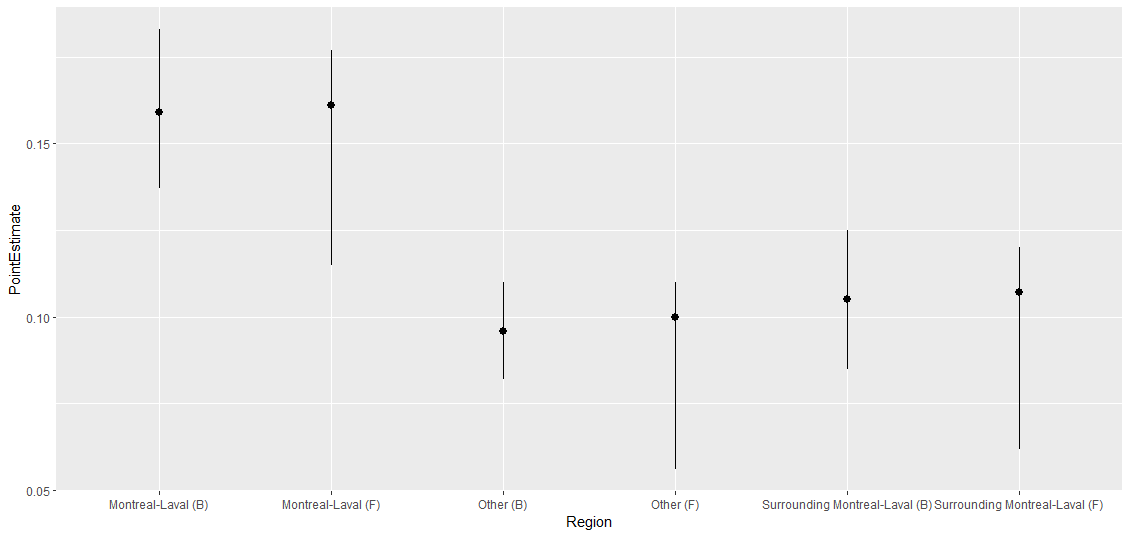
\includegraphics[width=\columnwidth]{../../plot/intervals.png}
    \caption{Comparison between uncertainty intervals for regional cumulative incidences between the Bayesian (B) and non-Bayesian (F) seroprevalence analyses adjusted for both seroreversion and test-kit performance.}
    \label{fig:intervals}
\end{figure}